\documentclass[10pt,twoside]{article}                           % Twoside para poder poner números en lados alternados

\usepackage[spanish,es-tabla]{babel}                                     % Configuración de lenguaje
\usepackage[a4paper,top=2cm,bottom=2cm,left=3cm,right=3cm,marginparwidth=1.75cm]{geometry}          % Configurar tamaño de pagina y márgenes
%\usepackage[a4paper, top=2cm, bottom=2cm, outer=0cm, inner=0cm]{geometry}
\usepackage{fancyhdr}
\usepackage[autostyle=true]{csquotes}
\usepackage[backend=biber,sorting=none]{biblatex}               % Paquete para bibliografía 
\addbibresource{Bibliografia.bib}                               % Llamo al archivo que contiene las referencias
\usepackage{amsmath}
\usepackage{amsfonts}
\usepackage{makecell}                                           % Para poder poner line breaks en tablas
\renewcommand\cellgape{\Gape[4pt]}
\usepackage{caption}                                            % Para que "Figura x.y" este en bold
\usepackage{eso-pic}                                            % Para poder poner imágenes de fondo
\usepackage{multicol}                                           % Para multiples columnas
\usepackage{array, multirow}
\usepackage{moresize}                                           % Para tener texto de tamaño \HUGE
\usepackage{graphicx}
\usepackage{lipsum}
\usepackage[hidelinks]{hyperref}                                % Para links entre partes del documento (hidelinks no le cambia el color a los links)
\usepackage{float}                                              % Permite forzar una posición para una figura
\usepackage[justification=centering,labelsep=space]{caption}    % Para poder centrar captions de figuras
\usepackage{gensymb}                                            % Símbolo de grados (\degree)
\usepackage{subfigure}                                          % Para poder usar subfiguras (logos de UNLP y FI juntos)
\usepackage{listings}                                           % Para poder incluir código
\usepackage{xcolor}                                             % Para poder definir colores  
\usepackage{enumitem}                                           % Para poder poner letras como items de listas
\usepackage{afterpage}                                          % Para poder insertar pagina en blanco
\usepackage{titlesec}                                           % Para cambiar tamaño de headers de secciones, subsecciones, etc.
\usepackage{titletoc}                                           % Para modificar el aspecto del índice (Table of Contents - ToC)
\usepackage[pagecolor=none]{pagecolor}                          % Para permitir usar colores de fondo en páginas
\usepackage{siunitx}                                            % Para notación científica (y unidades SI)
\usepackage{mathspec}                                           % Para tipografías custom, incluyendo ecuaciones (Incluye fontspec)

%-------------------------------------------------------------------------------------------------------%

% Definir todas las tipografías de mathspec

\setmainfont{Montserrat}                                        % Letra principal
\newfontfamily\Thin{Montserrat Thin}                            % Defino todos los pesos, también se pueden definir tipografías adicionales de la misma manera
\newfontfamily\ExtraLight{Montserrat ExtraLight}
\newfontfamily\Light{Montserrat Light}
\newfontfamily\Medium{Montserrat Medium}
\newfontfamily\SemiBold{Montserrat SemiBold}
\newfontfamily\Bold{Montserrat Bold}
\setmonofont[Scale=1.1]{Fraunces 72pt Soft SemiBold}
\setmathrm[BoldFont = {Montserrat SemiBold Italic}]{Montserrat} 
\setmathfont(Digits,Latin){Montserrat}                          % Tipografía de matemática

% Comando para linea horizontal configurable que llene todo el espacio disponible 

\newcommand{\xfill}[2][1ex]{{%                                  % Si no hay texto antes del \xfill, hay que agregarle algun caracter como "\tiny\ " para que compile
  \dimen0=#2\advance\dimen0 by #1
  \leaders\hrule height \dimen0 depth -#1\hfill%
}}

% Comando para pagina en blanco sin numero de hoja

\newcommand{\ncblankpage}
{                          
    \null
    \thispagestyle{empty}
    \addtocounter{page}{-1}                         % No aumenta el contador de páginas
    \newpage
}



\newcommand{\blankpage}                             % Aumenta el contador de páginas
{                          
    \null
    \thispagestyle{empty}
    \newpage
}

% Definición de colores

\definecolor{AzulFI}{rgb}{0, 0.394, 0.645}                  % 0064A5
\definecolor{AzulFI_dark}{rgb}{0, 0.2353, 0.3882}           % 003C63
\definecolor{AzulFI_darker}{rgb}{0, 0.196, 0.3216}          % 003252
\definecolor{AzulFI_light}{rgb}{0.898, 0.9373, 0.9647}      % E5EFF6
%\definecolor{codegreen}{rgb}{0,0.6,0}
%\definecolor{codegray}{rgb}{0.5,0.5,0.5}
%\definecolor{codepurple}{rgb}{0.58,0,0.82}
%\definecolor{backcolour}{rgb}{0.95,0.95,0.92}

% Estilo del header y footer

\pagestyle{fancy}

\renewcommand{\sectionmark}[1]{\markright{#1}}                          % Borra el numero de sección de \rightmark            
\renewcommand{\subsectionmark}[1]{}                                     % No marca las subsecciones

% Estilo nuevo
\fancyfoot[CO]{\SemiBold%
    \rule[-0.2em]{1pt}{1.1em}\hspace{0.5em}%
    \color{AzulFI_dark}Tomás Tavella\hspace{0.5em}\normalcolor\rule[-0.2em]{1pt}{1.1em}%
    \hspace{-0.05em}\xfill[0.6ex]{1pt}\hspace{-0.05em}%
    \rule[-0.2em]{1pt}{1.1em}\color{AzulFI_dark}\hspace{0.5em}\thepage\normalcolor\hspace{0.5em}\rule[-0.2em]{1pt}{1.1em}%
}

\fancyfoot[CE]{\SemiBold%
    \rule[-0.2em]{1pt}{1.1em}\hspace{0.5em}\color{AzulFI_dark}\thepage\hspace{0.5em}\normalcolor\rule[-0.2em]{1pt}{1.1em}%
    \hspace{-0.05em}\xfill[0.6ex]{1pt}\hspace{-0.05em}%
    \rule[-0.2em]{1pt}{1.1em}\color{AzulFI_dark}\hspace{0.5em}Tomás Tavella\normalcolor\hspace{0.5em}\rule[-0.2em]{1pt}{1.1em}%
}

\fancyhead[C]{\SemiBold%
    \rule[-0.2em]{1pt}{1.1em}\hspace{0.5em}\scshape\color{AzulFI_dark}Capítulo \thesection\normalcolor\hspace{0.5em}\rule[-0.2em]{1pt}{1.1em}%
    \hspace{-0.05em}\xfill[0.6ex]{1pt}\hspace{-0.05em}%
    \rule[-0.2em]{1pt}{1.1em}\color{AzulFI_dark}\hspace{0.5em}\rightmark\normalcolor\hspace{0.5em}\rule[-0.2em]{1pt}{1.1em}%
    }

\fancyhead[R,L]{}

\renewcommand{\headrulewidth}{0pt}
\setlength{\headheight}{12.60013pt}

\fancypagestyle{plain}{
    \fancyhead[L,C,R]{}
    %\fancyfoot[C]{}                                                    % Sólo va con el estilo viejo
    \renewcommand{\headrulewidth}{0pt}                                  % Para que no haya linea horizontal de encabezado en las páginas de índice y título de sección
}

% Parametros para setear como se muestra el codigo

\lstdefinestyle{mystyle}{                       
    backgroundcolor=\color{backcolour},
    commentstyle=\color{codegreen},
    keywordstyle=\color{magenta},
    numberstyle=\tiny\color{codegray},
    stringstyle=\color{codepurple},
    basicstyle=\ttfamily\scriptsize,
    breakatwhitespace=false,         
    breaklines=true,                 
    captionpos=b,                    
    keepspaces=true,                 
    numbers=left,                    
    numbersep=5pt,                  
    showspaces=false,                
    showstringspaces=false,
    showtabs=false,                  
    tabsize=4
}

\lstset{style=mystyle}

% Macro para divisores horizontales

\newcommand{\divider}                           
{
\vspace{0.4cm}
\begin{center}
    \tiny\ \xfill[8pt]{1pt}\ \ \linebreak
\end{center}
%\vspace{0.25cm}
\normalsize
}

% Macro para usar colorbox en ecuaciones

\newcommand{\highlight}[1]{\colorbox{AzulFI_light}{$\displaystyle #1$}}

% Macro para comillas

\newcommand{\quotes}[1]{``#1''}                 % Comando para double quotes

% Números de figura y ecuación por seccion (1.1 , 2.1, etc.)

\numberwithin{figure}{section}                  % Numeros de figura por seccion
\numberwithin{equation}{section}                % Numeros de ecuacion por seccion
\numberwithin{table}{section}

% Definir formato de titulos de secciones y subsecciones

\titleformat{\section}[display]                                     % display permite el numero en linea separada del nombre
{\raggedright\color{AzulFI_dark}\scshape\Bold\Huge\centering}       % Formato del título de seccion
{\normalcolor\tiny\ \Huge\xfill[8pt]{1pt}\rule[-0.2em]{1pt}{1.1em}\hspace{0.5em}\color{white}\thesection\normalcolor\hspace{0.5em}\rule[-0.2em]{1pt}{1.1em}\xfill[8pt]{1pt}\tiny\ }{0.5em}{}       % Formato del número de seccion

\titleformat{\subsection}[hang]{\raggedright\color{AzulFI_dark}\scshape\huge\Bold}{\thesubsection\quad}{0.5em}{}                      % Se agrega raggedright a todos para que no separe palabras en dos cuando tiene que hacer un line break

\titleformat{\subsubsection}[hang]{\raggedright\color{AzulFI_dark}\scshape\Large\Bold}{\thesubsubsection\quad}{0.5em}{}
\titleformat{\paragraph}[hang]{\raggedright\color{AzulFI_dark}\large\SemiBold}{}{0.5em}{}
\titleformat*{\subparagraph}{\raggedright\SemiBold}

% Formato de captions de figuras

\DeclareCaptionFormat{custom}
{%
    \SemiBold\scshape\color{AzulFI_dark} #1#2 \normalfont\normalcolor \textit{#3}                     % #1 es el número, #2 el separador y #3 el texto
}
\captionsetup{format=custom}

% Formato de Table of Contents (ToC)

\contentsmargin{1em}
\dottedcontents{section}[1.5em]{\large\vspace{0.4cm}\Bold\scshape\color{AzulFI_dark}}{1.5em}{0pc}      % Secciones en Bold en TableofContents
\dottedcontents{subsection}[4em]{\vspace{0.1cm}\Medium}{2.5em}{0.6pc}
\dottedcontents{subsubsection}[7.5em]{}{3.5em}{0.6pc}

%---------------------------------------------------------------------------------------------------------%
%------------------------------------------ Inicio de Documento ------------------------------------------%
%---------------------------------------------------------------------------------------------------------%

\begin{document}

    \nocite{*}                                                      % Se usa para que aparezcan todas la referencias del .bib sin tener que citarlas en el texto

    \newgeometry{top=1.5cm,bottom=2cm,left=1cm,right=1cm,marginparwidth=1.75cm}
    %\newpagecolor{AzulFI}\afterpage{\restorepagecolor\blankpage}    % Página en blanco entre portada y agradecimientos
    

        \begin{titlepage}
        \begin{center}
            \vspace*{0.5cm}
            \Huge\scshape
            \color{white}
            \Bold{Diseño y Desarrollo de una Plataforma Experimental de Evaluación de Sistemas Híbridos Basados en Pilas de Combustible}    % Titulo
            \normalfont
            \\
            \vspace{0.5cm}
            \huge
            Proyecto Final                                       % Subtitulo
            \\
            %\divider
            \vspace{2cm}
            \Large\scshape
            \SemiBold{Autor:}
            \normalfont
            \\
            \large
            \vspace{0.2cm}
            Tomás Tavella
            \\
            N° 68371/4
            \\
            \vspace{1cm}
            \Large\scshape
            \SemiBold{Director:}
            \normalfont
            \\
            \vspace{0.2cm}
            \large
            Ing. Jorge Anderson Azzano
            \\
            \vspace{0.3cm}
            \Large\scshape
            \SemiBold{Co-Director:}
            \normalfont
            \\
            \vspace{0.2cm}
            \large
            Dr. Ing. Paul F. Puleston
            \\
            \vfill
            \begin{figure}[H]
                \centering
                \begin{subfigure}
                    \centering
                    
\includegraphics[width=0.25\textwidth]{Imagenes/UNLP.pdf}
                \end{subfigure}
                \begin{subfigure}
                    \centering
                    
\includegraphics[width=0.32\textwidth]{Imagenes/FI Invertido.png}
                \end{subfigure}
            \end{figure}
            \vspace{1cm}
            \SemiBold
            Facultad de Ingeniería
            \\
            Universidad Nacional de La Plata
            \vspace{1cm}
        \end{center}
    \end{titlepage}
    \restoregeometry\blankpage
    
    \addtocounter{page}{-1}
    \newpage 
    \thispagestyle{empty}                                           % Para que no se muestre el número de página al final (igual contribuye a la cuenta total)
    \afterpage{\ncblankpage}

    \huge
\scshape\color{AzulFI_dark}
\Bold{Agradecimientos}\\

\normalsize\normalfont\normalcolor
[Faltan los agradecimientos]

    \newpage
    \thispagestyle{empty}
    \afterpage{\blankpage}

    \huge
\scshape
\Bold{Resumen}\\

\normalfont\normalsize
Este trabajo consiste del estudio, diseño, implementación y validación de una plataforma experimental para la evaluación de sistemas híbridos de generación energía (SHGE) a partir de pilas o celdas de combustible de tipo PEMFC (\textit{Proton Exchange Membrane Fuel Cell}). Esta plataforma consiste en un sistema de conversión electrónico de tipo CC-CC conmutado y aislado, de topología puente completo; monitoreado mediante la medición de sus estados, y controlado por una excitación de tipo PWM (\textit{Pulse-Width Modulation}) provista por un DSC (\textit{Digital Signal Controller}) de alta performance. Este convertidor es requerido para poder adaptar la tensión variable que entrega una celda de combustible a una tensión de salida fija para conectar a un bus común de corriente continua.\\

En el desarrollo de este informe se detallan las tareas realizadas para cumplir este objetivo: el estudio y comprensión de las topologías de conversión CC-CC; la simulación de la topología elegida mediante herramientas de simulación circuitales; el diseño de circuitos auxiliares de excitación, sensado y protección; la implementación del sistema en una placa de circuito impreso mediante software EDA (\textit{Electronic Design Automation}); la programación de los algoritmos de control del sistema; y, finalmente la validación experimental de la plataforma.\\

\vspace{1cm}
\huge
\scshape
\Bold{Abstract}\\

\normalsize\normalfont
This work entails the study, design, implementation and validation of an experimental platform for the evaluation of hybrid energy generation systems based on Proton Exchange Membrane Fuel Cells (PEMFC). This platform incorporates a full-bridge isolated switched-mode DC-DC electronic converter, monitored via the measurement of its state variables, and controlled by a pulse-width modulated (PWM) signal, generated using a high-performance Digital Signal Controller (DSC). This converter provides the adaptation from the variable output voltage of the PEMFC to the fixed voltage of the common DC bus at the system output.\\

This report details the process through which the goals were achieved: study and understanding of the different DC-DC converter topologies, simulation of the selected converter topology using circuit simulation tools, design process of auxiliary circuits, including driver, sensing and protection circuits,  implementation of the system PCB (printed circuit board) through the use of electronic design automation (EDA) software, programming of system control algorithms, and experimental validation of the working platform.\\ 

    \newpage
    \afterpage{\blankpage} 
    \thispagestyle{plain}
    \tableofcontents
    \newpage

    \section{Introducción} \label{introduccion}
\AddToShipoutPictureBG*{
\includegraphics[width=\paperwidth,height=\paperheight]{Imagenes/Fondo Capitulo 1.pdf}}
\thispagestyle{plain}

\divider

Previo a comenzar con el diseño de la placa de circuito impreso, debemos introducir la plataforma que se tiene que plasmar en esta PCB, explicando brevemente su funcionamiento y los bloques principales y auxiliares que la componen. Se puede apreciar un diagrama de esta plataforma, separada en sus distintos bloques funcionales en la figura \ref{fig:plataforma}.\\

\begin{figure}[h]
    \centering
    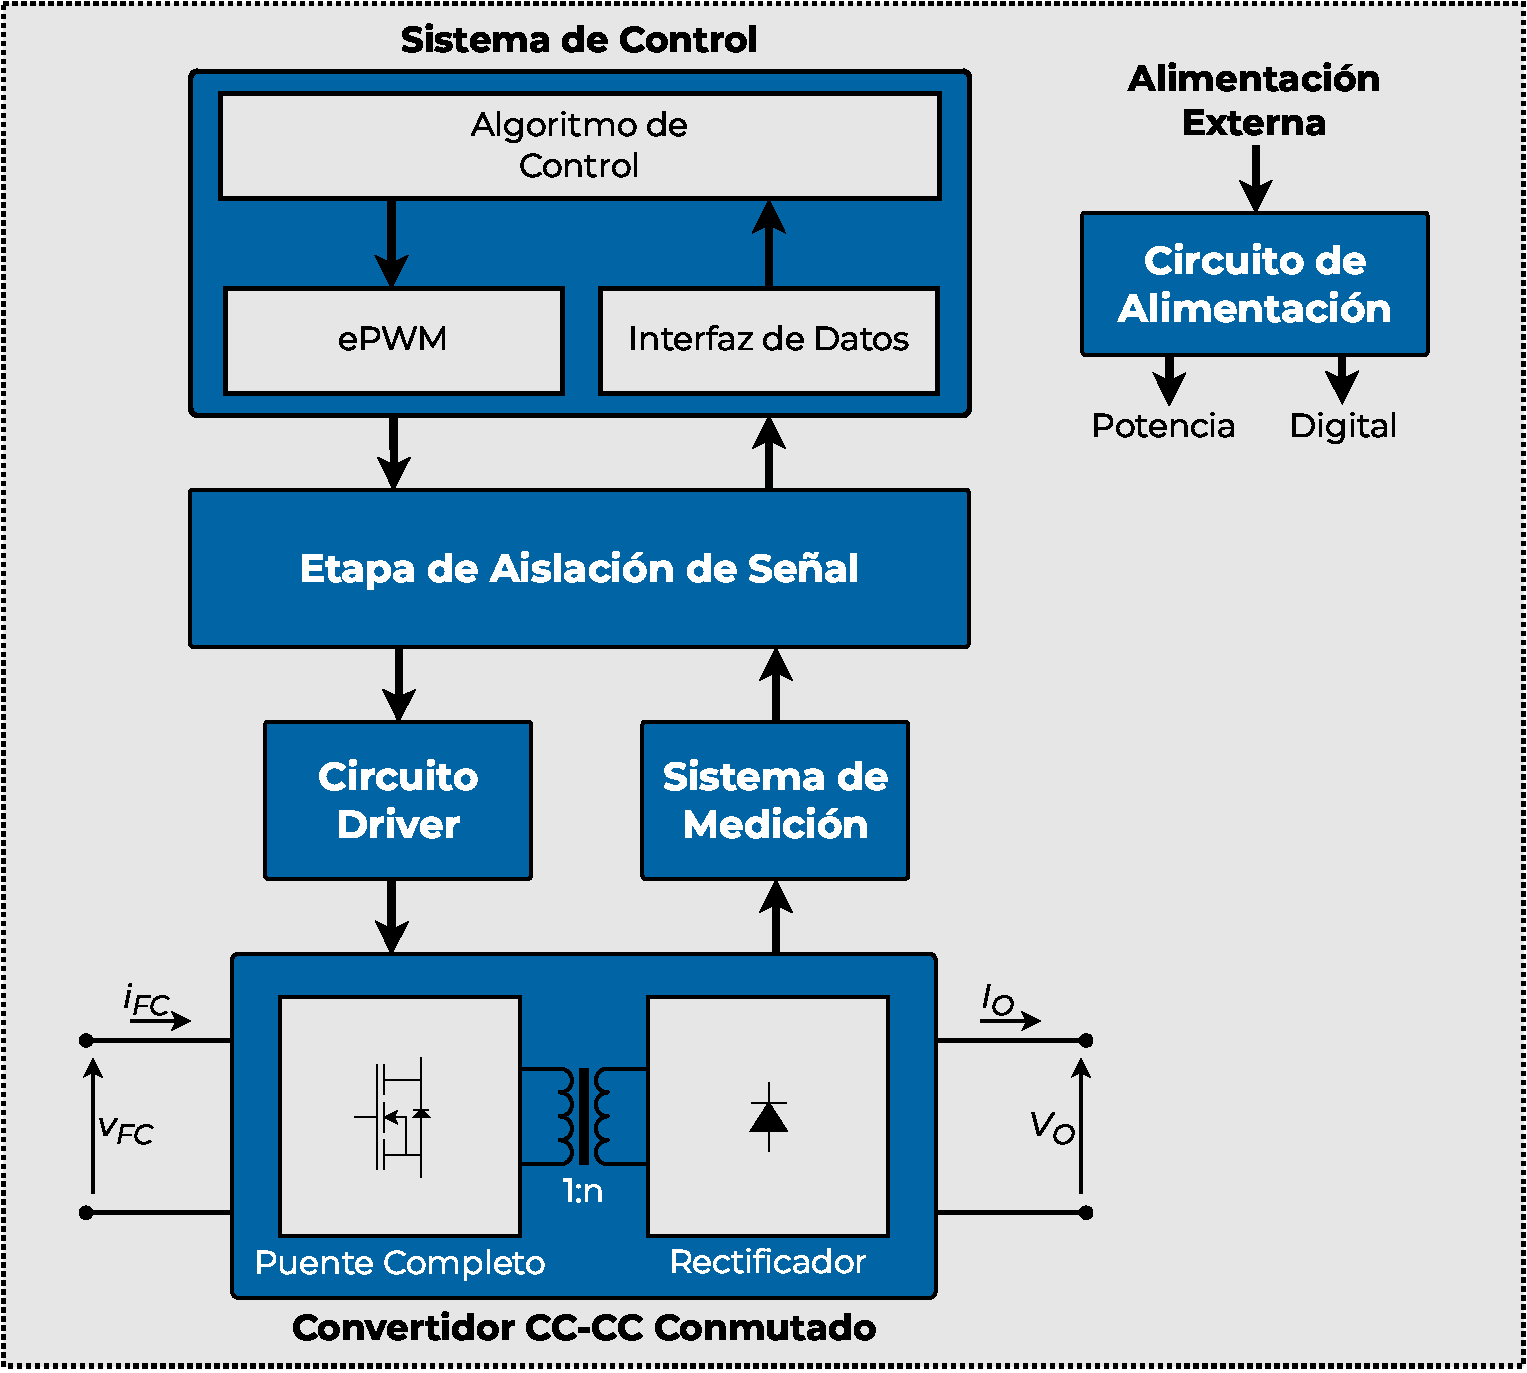
\includegraphics[scale=0.4]{Imagenes/Plataforma Detallada.pdf}
    \caption{Diagrama de la plataforma experimental de evaluación de celdas de combustible.}
    \label{fig:plataforma}
\end{figure}

Esta plataforma tiene como objetivo la adaptación de la interconexión de bloques en sistemas híbridos, sistemas complejos que combinan (o hibridan) múltiples módulos de generación y almacenamiento de energía, generalmente renovables, que luego se conectan a un bus de potencia de corriente continua (CC).\\

Particularmente, este sistema adapta el módulo de generación a partir de pilas de combustible para utilizar en un sistema híbrido, con una tensión de pila en la entrada $v_{FC}$ variable entre \SI[]{30}[]{\volt} y \SI[]{65}[]{\volt}, y una tensión de salida común fija de \SI[]{75}[]{\volt}. Para realizar esta la adaptación de estos niveles de tensión, se utilizó un convertidor CC-CC conmutado y aislado de tipo puente completo, que se regula mediante un sistema de control basado en un microcontrolador de tiempo real de la línea C2000 de Texas Instruments.\\

Previo a la realización de esta PPS, se trató el diseño circuital de la plataforma, construyendo los circuitos correspondientes a cada uno de los bloques que se muestran en la figura \ref{fig:plataforma}. Con estos circuitos diseñados, nos es posible pasar a su implementación en la placa de circuito impreso.\\

    \newpage
    \thispagestyle{plain}
    \printbibliography[heading=bibintoc,title={Referencias}]
    \thispagestyle{plain}
    
\end{document}